\chapter{Analiza aplikacji}
\label{cha:analizaAplikacji}

\section{Diagram przypadków użycia}
\label{sec:przypadkiUzycia}
\noindent
\begin{minipage}{\linewidth}
\makebox[\linewidth]{
  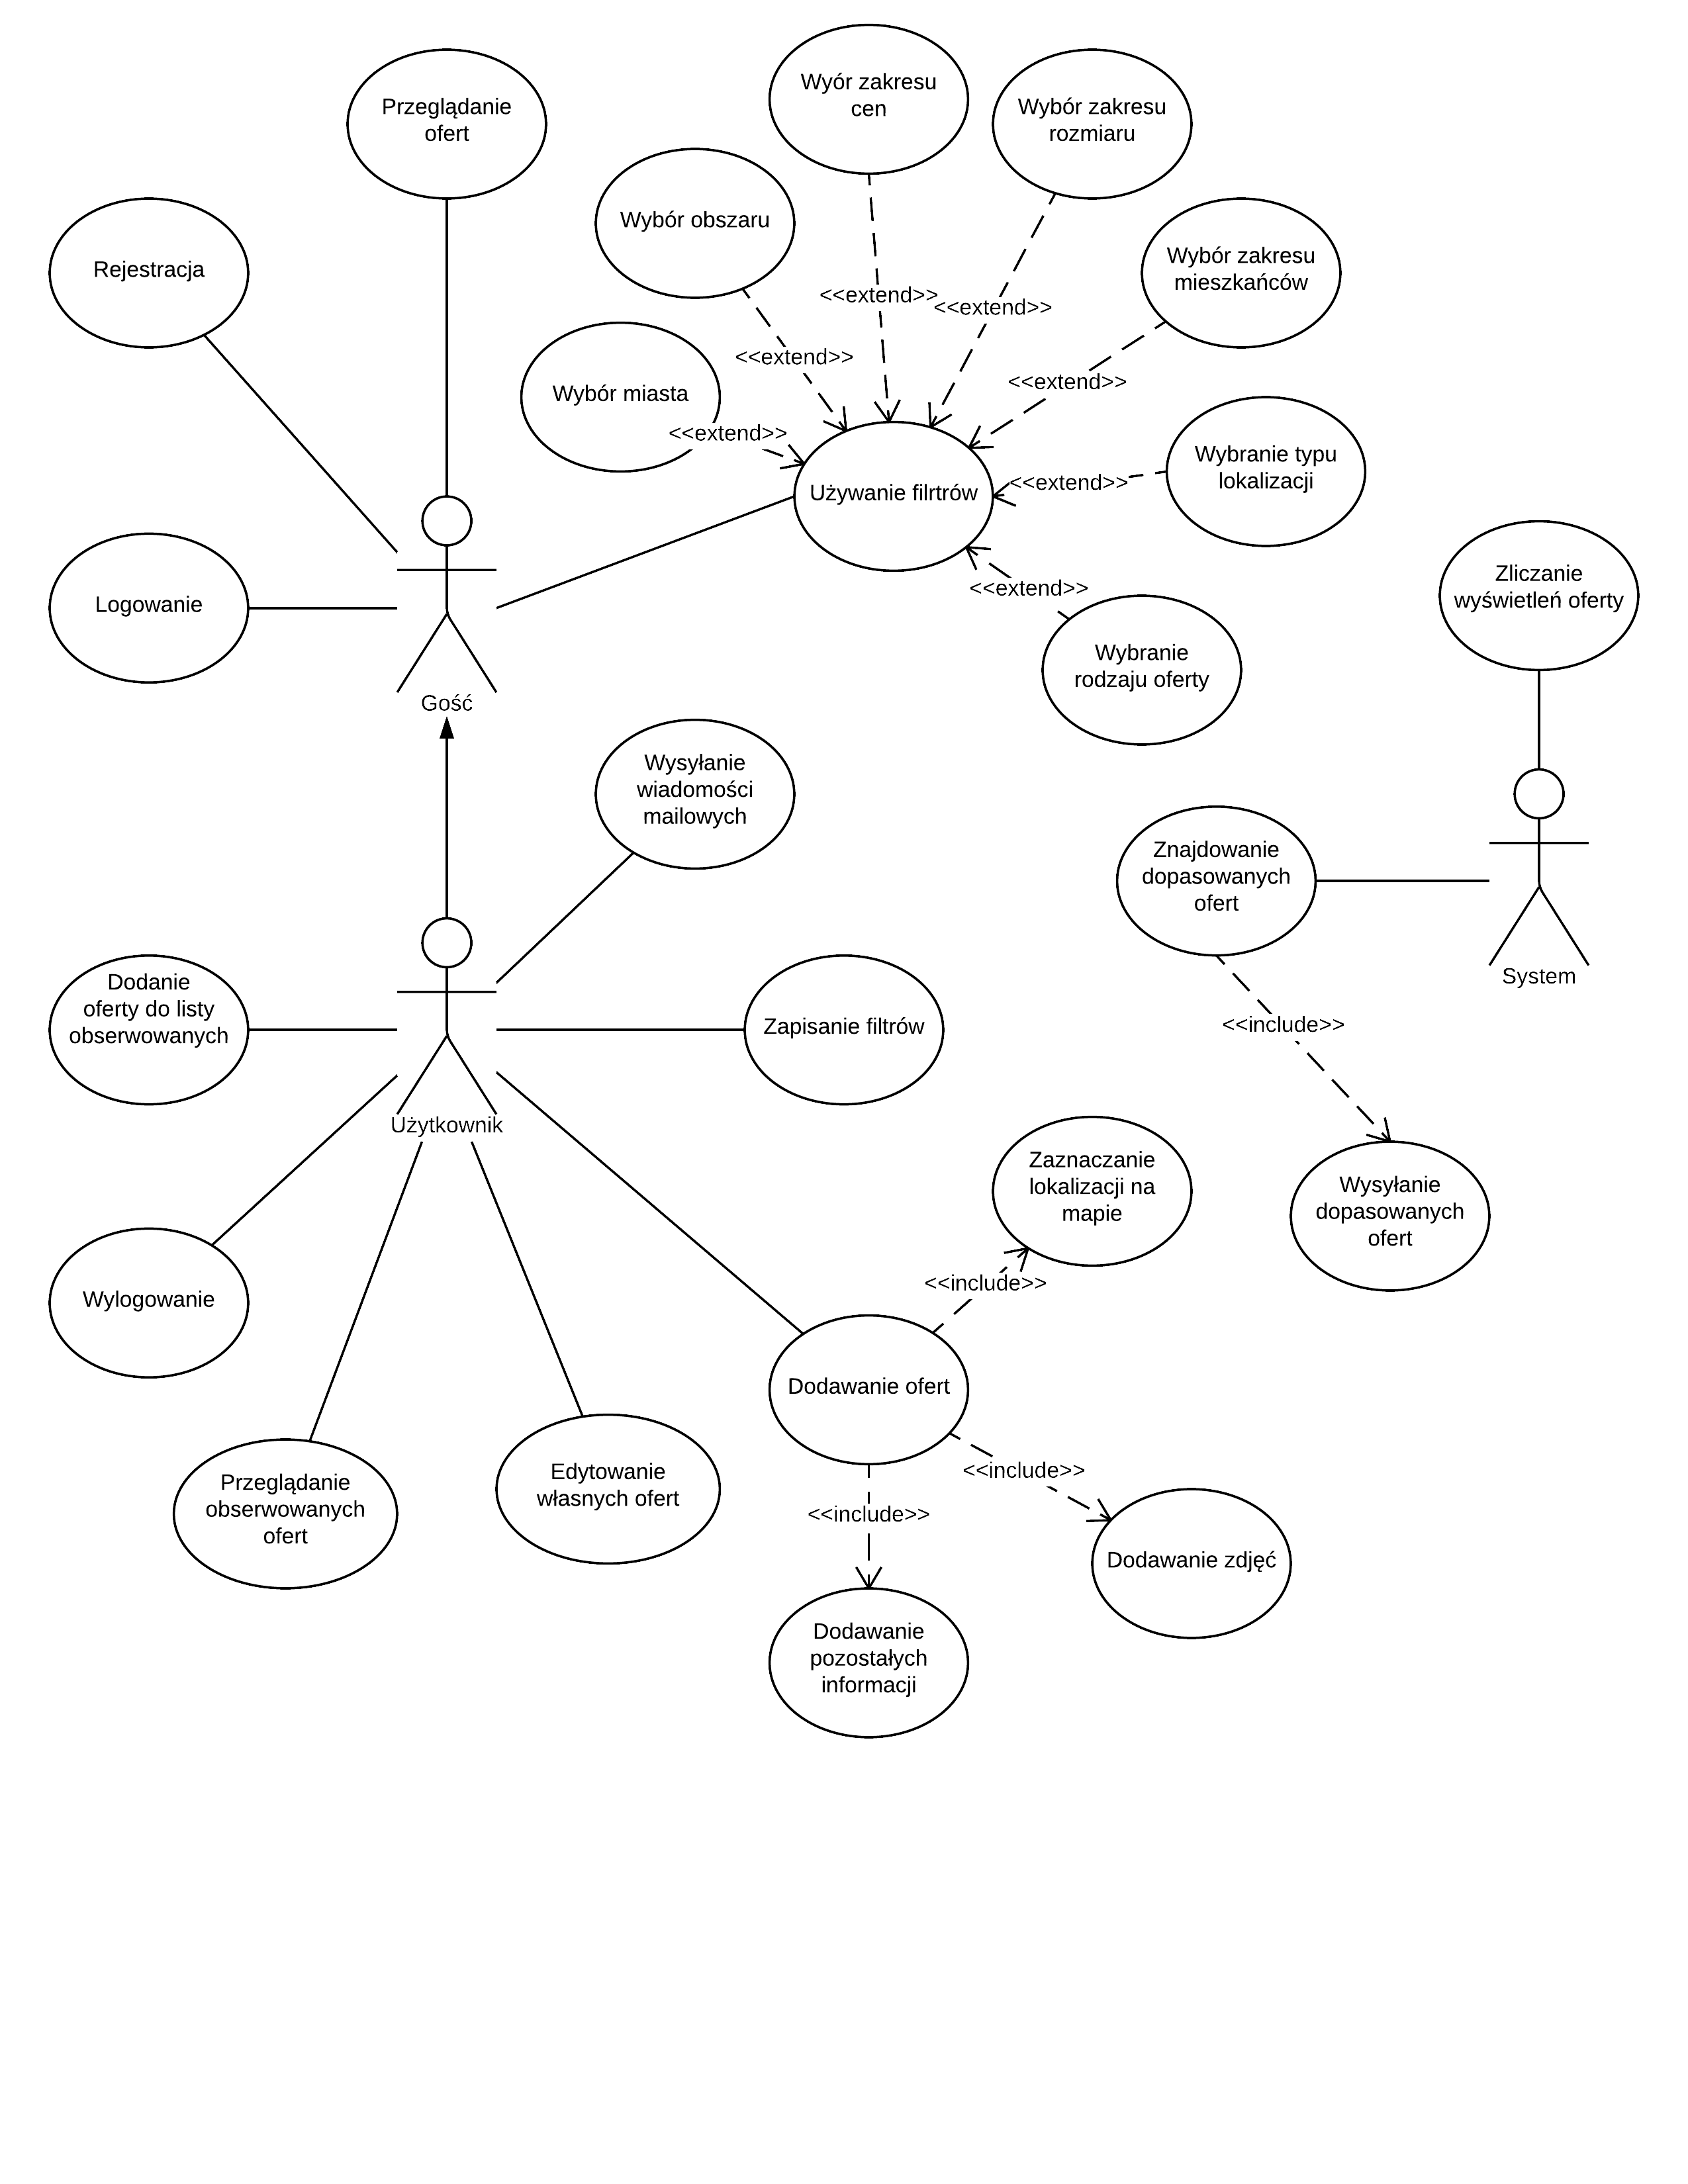
\includegraphics[keepaspectratio=true,scale=0.75]{pictures/use-case.png}}
\captionof{figure}{Diagram przypadków użycia}\label{use-case}
\end{minipage}

\section{Model bazy danych}
\label{sec;modelBazyDanych}

\noindent
\begin{minipage}{\linewidth}
\makebox[\linewidth]{
  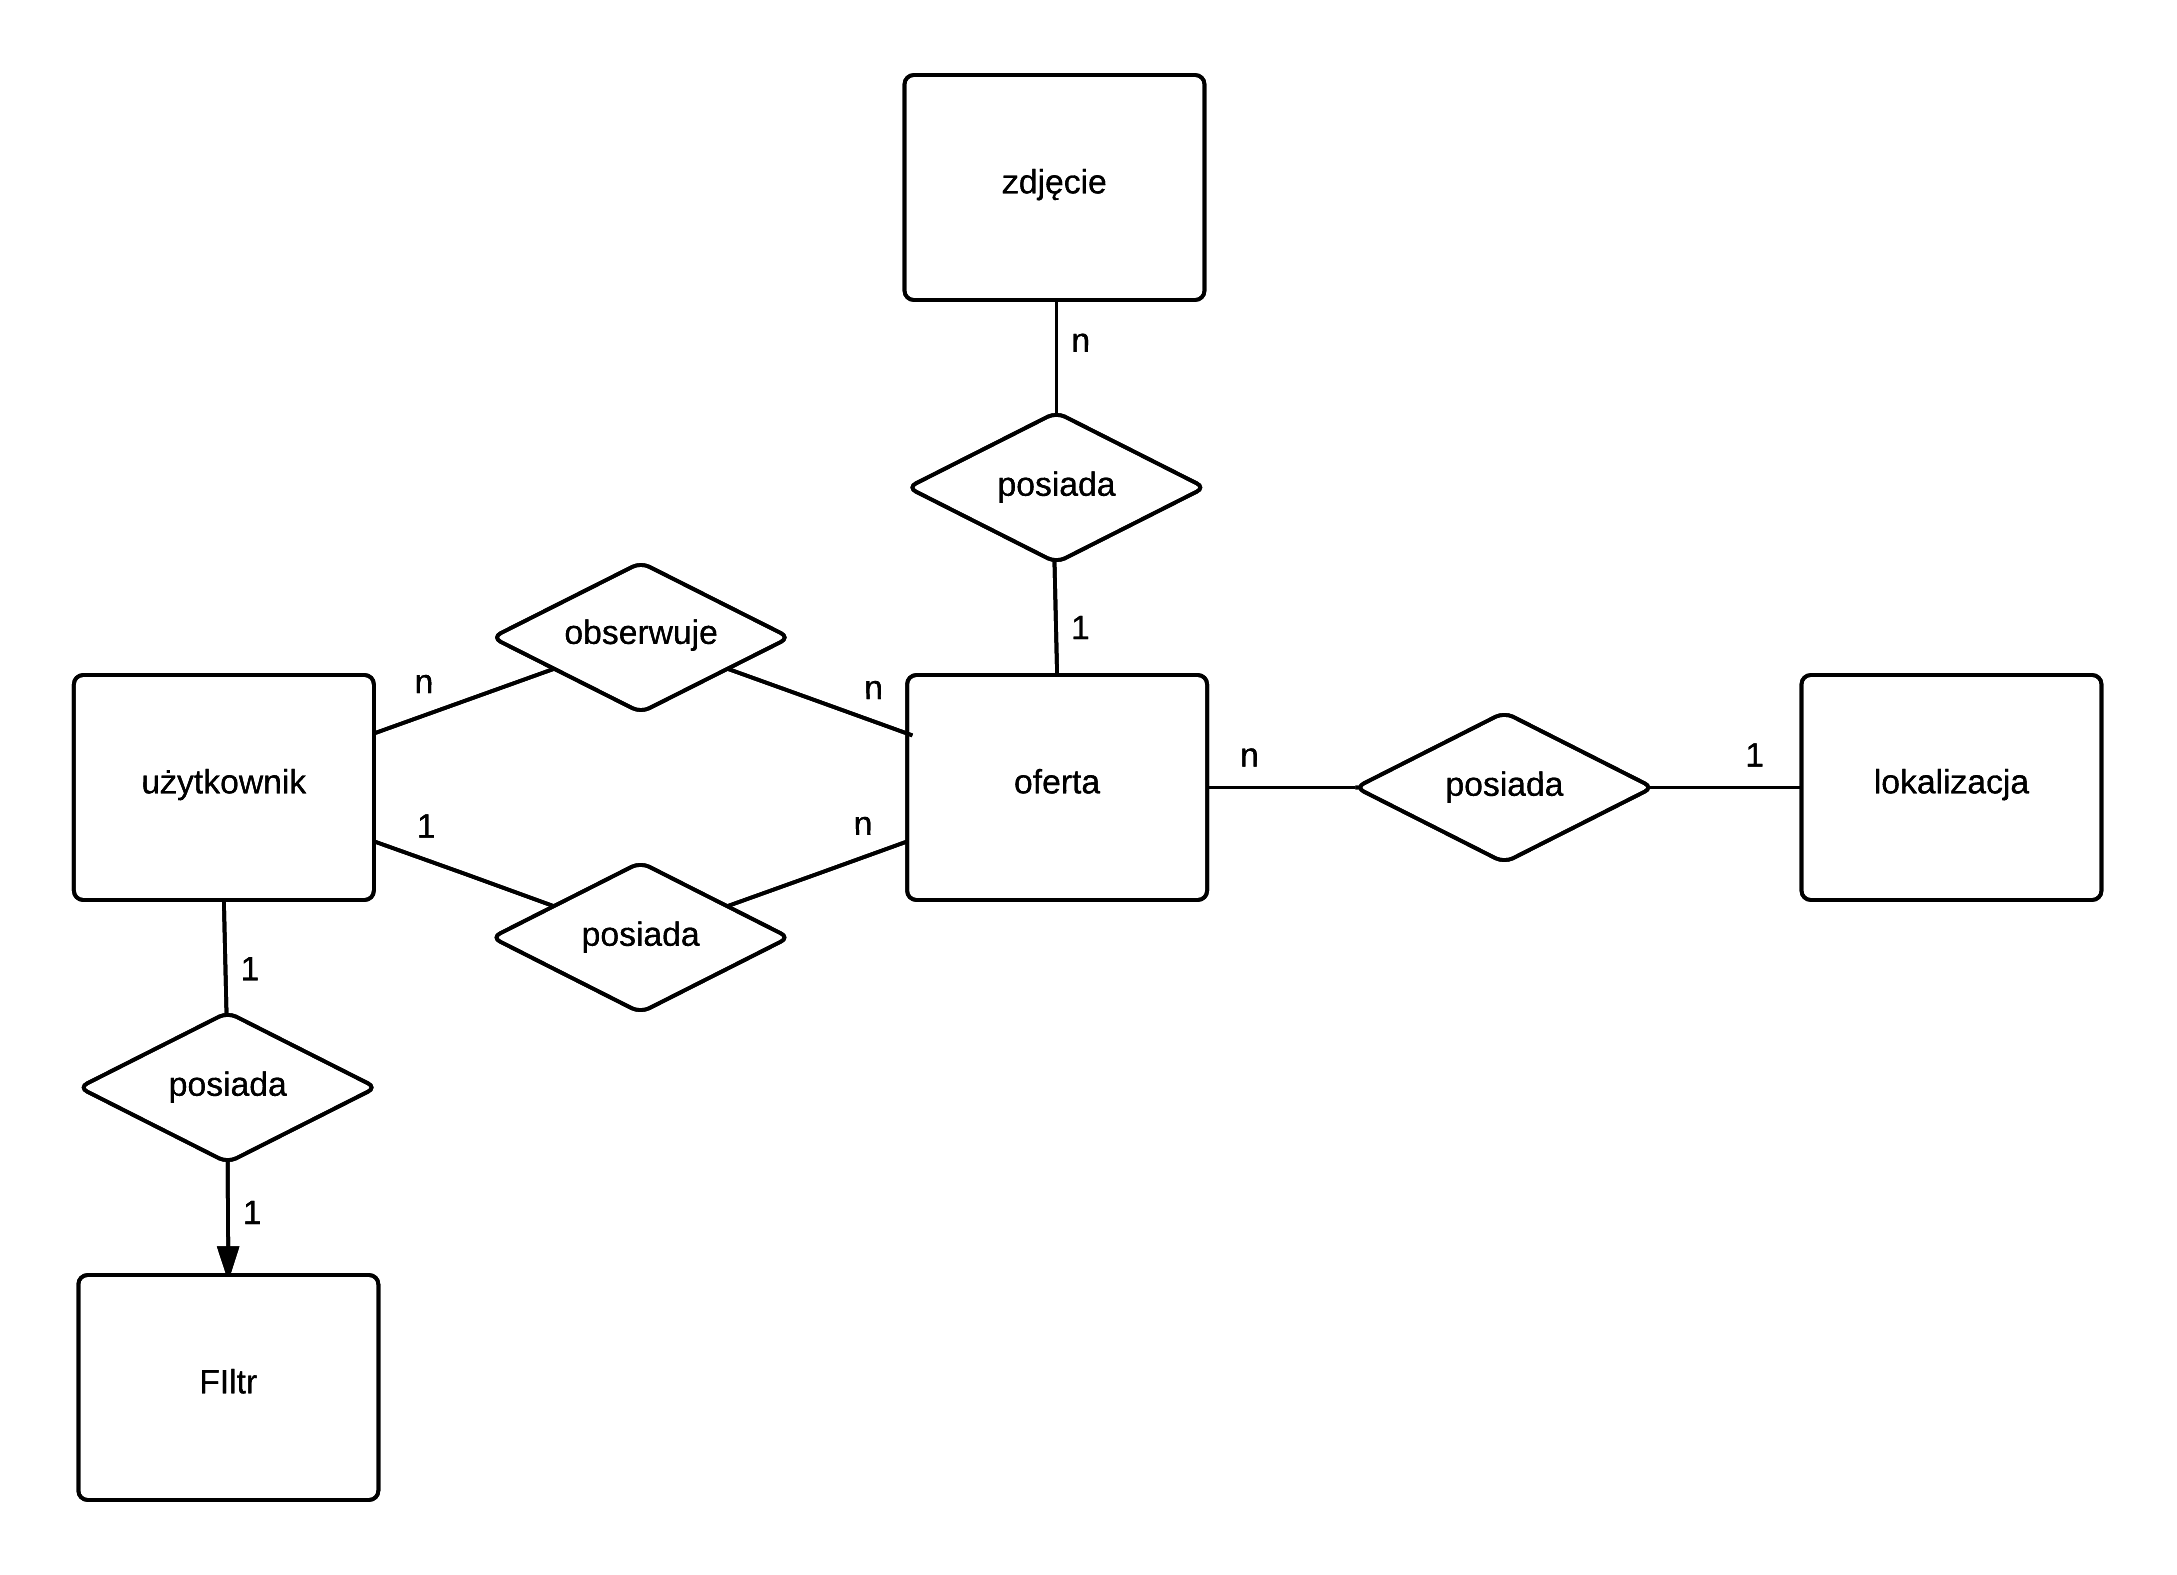
\includegraphics[keepaspectratio=true,scale=0.9]{pictures/erd.png}}
\captionof{figure}{Diagram ERD bazy danych}
\end{minipage}

\section{Opis struktury danych oferty}
\label{sec:strukturaOferty}
Kluczową strukturą dla poprawnego działania całego programu jest struktura oferty. Jest to bardzo rozbudowany model, lecz było to konieczne ze względu na dużą liczbę atrubutów którymi oferty muszą być opisane. Atrybuty oferty można podzielić ze względu na typ:
\begin{itemize}
\item Numeryczny całkowity
\begin{itemize}
\item size - rozmiar mieszkania w metrach kwadratowych
\item rooms - liczba pokoi
\item people - liczba osób mogących mieszkać w danej lokalizacji
\item floor - piętro budynko
\item views - liczba wyświetleń oferty
\end{itemize}
\item Znakowy
\begin{itemize}
\item offer\_type - typ oferty
\begin{itemize}
\item O - od właściciela
\item A - od agencji mieszkaniowej
\end{itemize}
\item location\_type - typ lokalizacji 
\begin{itemize}
\item H - dom
\item F - mieszkanie
\item R - pokój
\end{itemize}
\item building\_type - typ budynku
\begin{itemize}
\item H - dom
\item T - kamienica
\item A - blok
\end{itemize}
\item parking\_type - typ parkingu
\begin{itemize}
\item N - brak możliwości zaparkowania auta
\item R - istnieje możliwość ale miejsce nie jest gwarantowane
\item O - miejsce gwarantowane niezadaszone
\item G - miejsce w garażu
\end{itemize} 
\item heating\_type - typ ogrzewania
\begin{itemize}
\item G - gazowe
\item E - elektryczne
\item C - Centralne - opał stały
\item D - ogrzewanie miejskie
\end{itemize}
\end{itemize}
\item Numeryczny niecałkowity
\begin{itemize}
\item parking\_price - cena za parking
\item media\_price - opłata za wodę, prąd, internet itd.
\item rent\_price - kwota odstępnego dla właściciela 
\item sum\_price - kwota całkowita
\item bail - kaucja
\end{itemize}
\item Logiczny
\begin{itemize}
\item animals - czy są dozwolone zwierzęta
\item students - czy osoby wynajmujące mogą być studentami
\item basement - czy nieruchomość posiada piwnicę
\item balcony - czy nieruchomość posiada balkon
\item elevator - czy w budynku jest winda
\item internet - czy jest dostępny internet w mieszkaniu
\item cigaretts - czy w mieszkaniu można palić tytoń
\end{itemize}
\item Data
\begin{itemize}
\item from - od kiedy nieruchomość jest dostępna
\end{itemize}
\end{itemize} 
Można również zauważyć, że oferta posiada klucz obcy do tabeli locations. Tabela locations zawiera podstawowe dane adresowe. Zastosowana została tutaj relacja jeden do jednego w celu ograniczenia rozmiaru tabeli offers oraz rozgraniczenia logicznego modeli.\\
Równie obszerny model to tabela filters. Nie zostanie jednak omówione w pracy jej atrybuty, gdyż są bardzo podobne do atrybutów modelu offers.
\section{Architektura aplikacji}
\label{sec:architektura}
\noindent
\begin{minipage}{\linewidth}
\makebox[\linewidth]{
  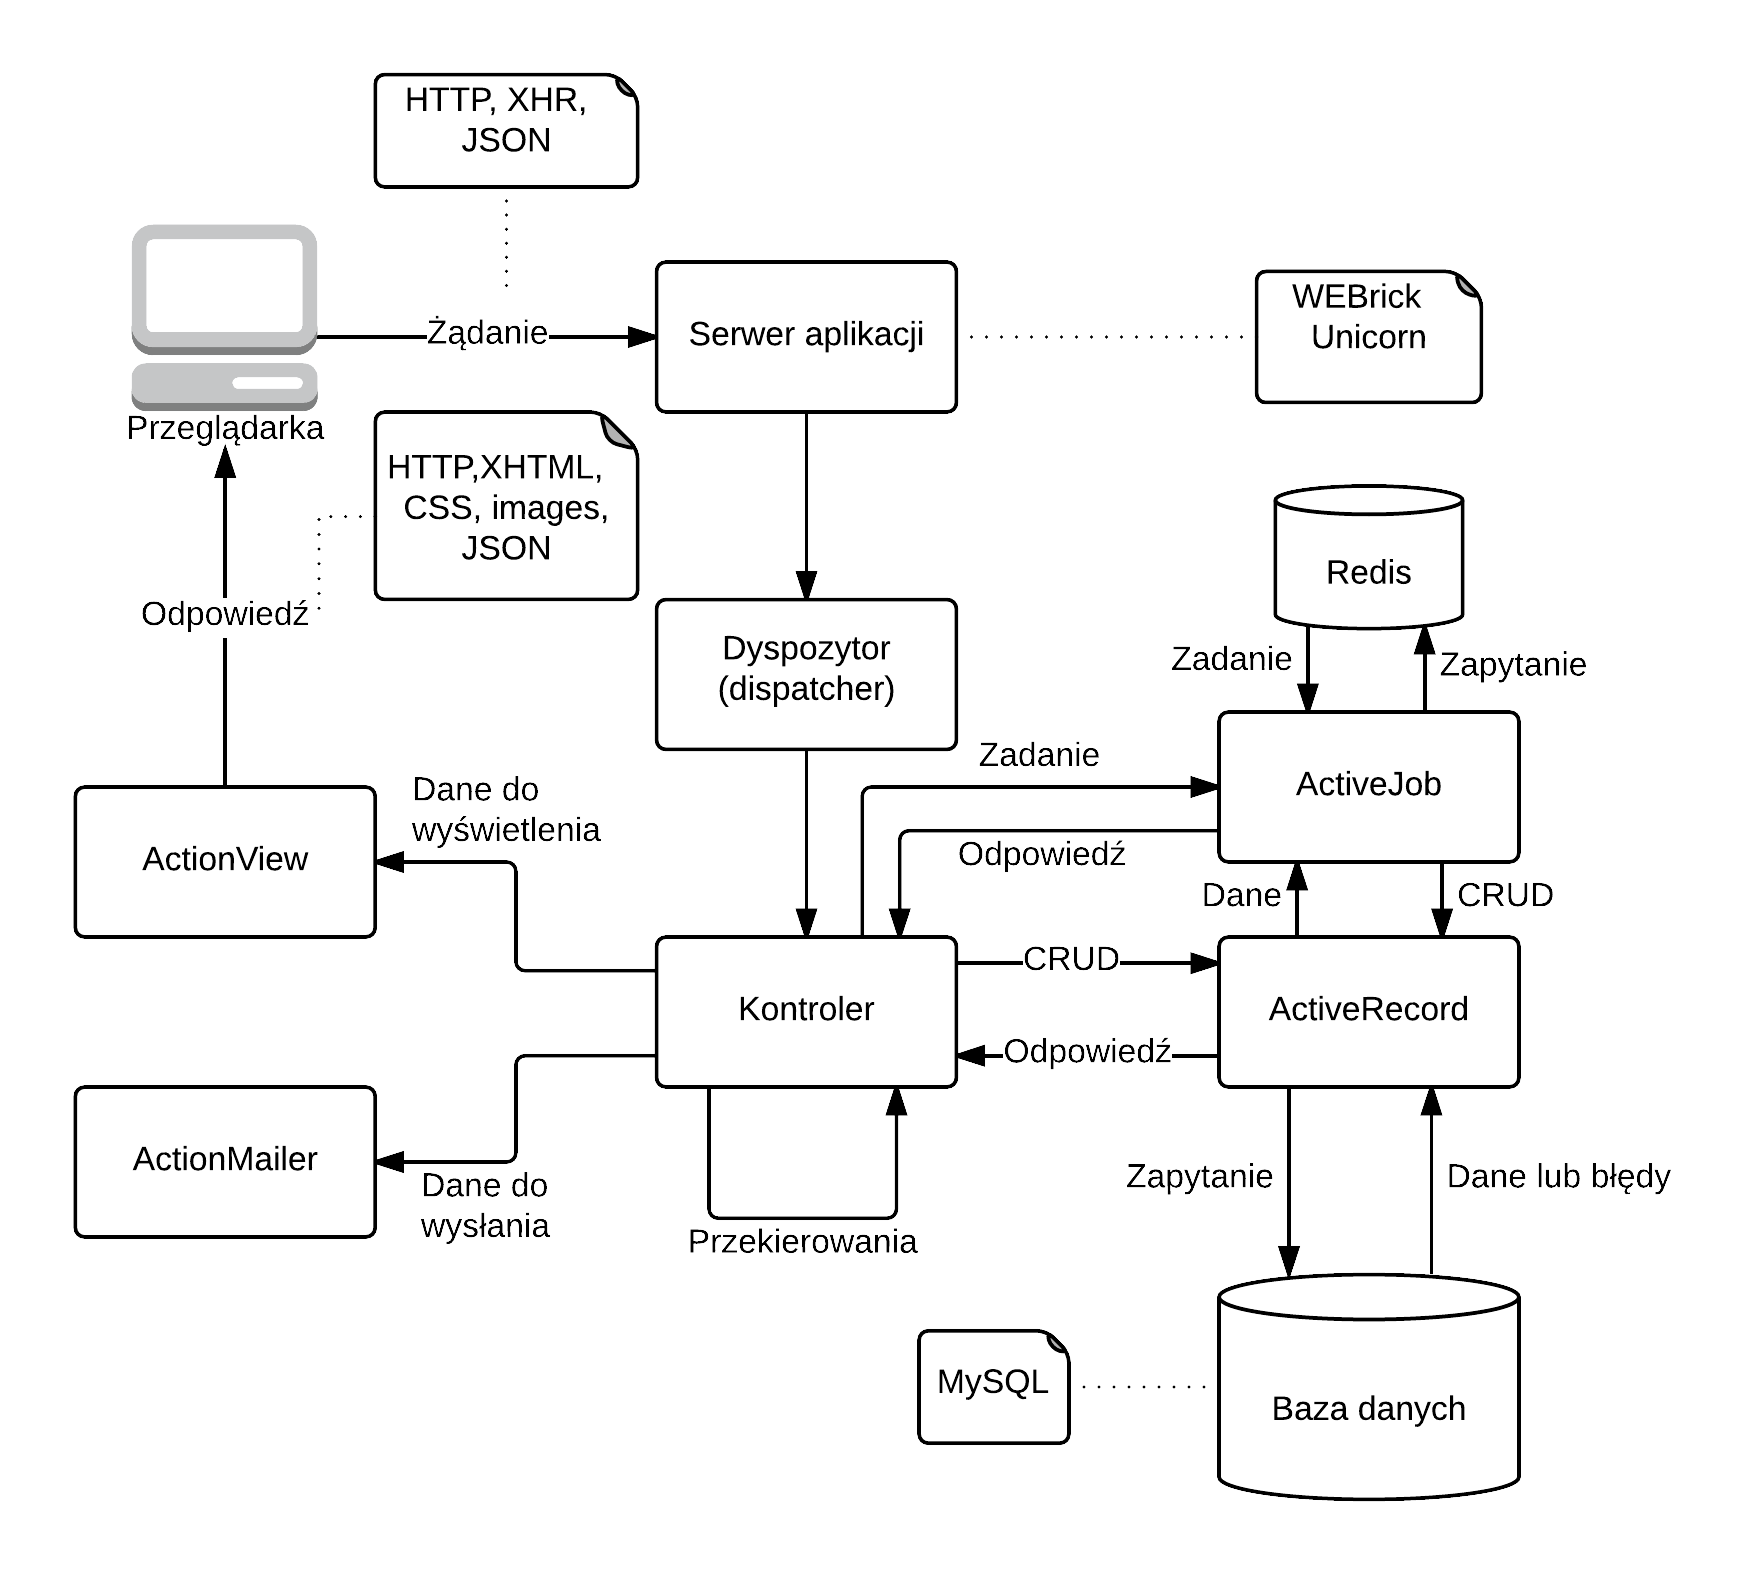
\includegraphics[keepaspectratio=true,scale=0.9]{pictures/architecture.png}}
\captionof{figure}{Diagram architektury}\label{use-case}
\end{minipage}
